\section{Introduction}
To evaluate the modified methods, a dataset and a trained model where we can apply the methods is required.

The constituent proposed the BraTS \cite{menze2015multimodal} dataset. This dataset contains
images of human brains taken with an MRI machine. The images are taken from patients which have brain tumors of the glioblastoma type or lower grade glioma type. The dataset contains four different types of images taken by MRI called modalities. 

Figure \ref{brats_example} shows the four modalities.

\begin{figure}[H]
    \centering
    \begin{subfigure}[t]{.2\textwidth}
        \centering
        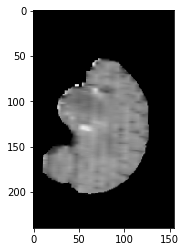
\includegraphics[width=\linewidth]{chapters/04_segmentation/images/brats/0.png}
        \caption{T1 modality}
    \end{subfigure}%
    \begin{subfigure}[t]{.2\textwidth}
        \centering
        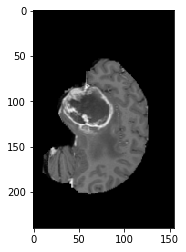
\includegraphics[width=\linewidth]{chapters/04_segmentation/images/brats/1.png}
        \caption{T1 contrast enhanced modality}
    \end{subfigure}%
    \begin{subfigure}[t]{.2\textwidth}
        \centering
        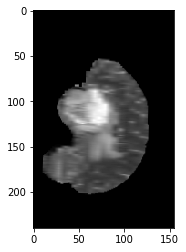
\includegraphics[width=\linewidth]{chapters/04_segmentation/images/brats/2.png}
        \caption{T2 modality}
    \end{subfigure}%
    \begin{subfigure}[t]{.2\textwidth}
        \centering
        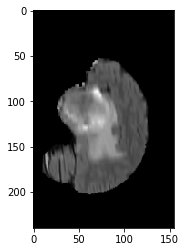
\includegraphics[width=\linewidth]{chapters/04_segmentation/images/brats/3.png}
        \caption{FLAIR modality}
    \end{subfigure}%
    \begin{subfigure}[t]{.2\textwidth}
        \centering
        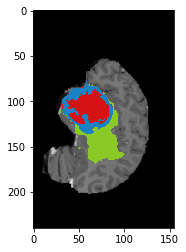
\includegraphics[width=\linewidth]{chapters/04_segmentation/images/brats/4.png}
        \caption{Tumor segment}
    \end{subfigure}
    \caption{The first four images show the modalities of the MRI scans in the BraTS dataset. Image (e) shows the tumor segmentation ground truth.}
    \label{brats_example}
\end{figure}

In addition, the dataset contains ground truth labels as seen in image (e) of Figure \ref{brats_example}. These labels mark the region in the brain where the tumor resides. This segments further differentiates between three different tissue types of the tumor: Gadolinium-enhancing tumor (ET), peritumoral edema (ED) and necrotic and non-enhancing tumor core (NCR/NET). Enhancing and non-enhancing in this context means if this tissue type is better visible when giving the patient a contrast enhancing fluid before making the MRI scans. These labels were manually drawn by physicians and validated by experienced neuro-radiologists.
The labels are saved in the same format as the scanner images, every type of tissue uses a specific integer value saved in the label file.
